\documentclass[a4paper]{article}
\setcounter{secnumdepth}{0}
\usepackage[english]{babel}
\addto\captionsenglish{
	\renewcommand{\contentsname}%
	{Table of Contents}%
}
\renewcommand\familydefault{\sfdefault}
\usepackage{graphicx}
\usepackage{subcaption}
\usepackage[margin=2cm]{geometry}
\renewcommand{\thesubsection}{\thesection\alph{subsection}}
\title{\vspace{-2.0cm}Summer Research Scholarship Report \\ 
		Teddy}
\author{Habit-Based Lego Robot\\
		Supervised by Matthew Egbert\\[10pt]
		Student 1: Teddy Halim \\ 
		Bachelor of Science in Computer Science \\
		Student 2: Darius Au \\
		Bachelor of Engineering in Software Engineering \\[10pt]
		Department of Computer Science \\
		University of Auckland}
\begin{document}
\maketitle
\tableofcontents
\section{Brief Statement}
This scholarship has challenged me to think critically in ways that I have never imagined before. It has helped me to always question everything even the most obvious one. Matthew Egbert has been a great supervisor and has always been guiding us through the whole project without fail. I also got to learn some new tools that I am sure will be helpful for my future career in this field. It has also pique my interest in research since I always thought that doing research is boring. After doing this project, I feel like I might want to do some research in the future just to see if I can get anything out of it.
\section{Summary}
This whole project is based on previous work by our supervisor, Matthew Egbert, and we follow it up by making a wireless connection, and also collecting and analysing the data which he had not done before. The entirety of this project has been dedicated to model or visualise the data collected to see, if any, some useful insight that we cannot determine just by observing. The project in itself has a big and far end goal and what we did so far has only been a fraction of what needs to be done to find some definite conclusion about this topic.
\newpage
\section{Abstract}
The purpose of this project was to understand the sensorimotor theory with the help of a simple agent, which is a LEGO MINDSTORMS EV3 robot. The idea first was to establish how do we even start relating both the robot and theory in a way that we can understand and make sense of. The basic idea of the theory is that how will both motor and sensor affect each other rather than only sensor affecting how the motor works. The project ran for ten weeks during the summer of 2017-2018. We first need to establish wireless communication between the robot and our dedicated computer to control the robot and also collecting the data to be analysed further. We use Ev3dev software \cite{ev3dev} and programming language that we choose is Python \cite{ev3devWithPython}. Our overall approach is to gather data from the robot and do some analysis and modelling on the data. There is a larger scope of this project than that which can be done in 3 months. 

\section{Simulation}
\subsection{Setting Up}
The Ev3dev Mindstorm LEGO robot has six values, two light sensors, two ultrasound sensors and two motors. It comes with a USB cable which we can use to connect both the robot and computer to make a wired network connection for the robot. We can then SSH into the robot and run any python script, sending it with \emph{scp command} from a terminal when the robot is online and connected to a network. We can already see the problem where if the robot moves, it is going to be constrained by the USB cable length. To solve this, we need to make a wireless connection between robot and computer. 
\\\newline
First of all, we need a USB Wi-Fi dongle for the robot to connect to University Wi-Fi. After plugging it in, we need to insert a new .config file, which consists of the credentials needed for the University Wi-Fi, in the \emph{connman folder} in the robot. Once this credential is inserted into the robot, we should be able to connect automatically to the University Wi-Fi after rebooting the robot. To test it, we can try to SSH into the robot using IPv4 shown on the top left corner of the Ev3dev robot. If everything works, you should be able to connect and access the robot wirelessly without the USB cable.
\subsection{Client-Server}
After wireless connection is established, the next step is to make the robot a client and our computer a server. This can be achieved by using socket over TCP and IPv4. We also incorporate multithreading into our client-server architecture to run multiple things simultaneously. On the server, we have two threads where one is to send the command to the client, and the other is to receive the data from the client and writing it to CSV output file. Meanwhile, on the client side, there are also two threads where one is to receive the command sent from the server, and the other is to collecting and sending the data from the client to the server.
\\\newline
There are multiple types of movement that the server can send as a command to the client. We have a manual control which uses keyboard and WASD key as moving forward, back, left, right respectively. There is also an autonomous robot movement which we got from our supervisor, Matthew Egbert, called a Braitenburg movement. All of the data such as light sensor, ultrasound sensor and motor value produced by the robot while moving is sent to the server in packages of 10 since we do not want to overload the socket with values.
\subsection{Experiment}
After all that set up and the client-server architecture is up, we can already run the robot in a controlled environment, or we called it arena so that we can collect the data properly. For clarification, the robot is attracted to any source of light and will move towards it while avoiding obstacle if one of the ultrasound sensors detect something is in front of it. One example of an arena is as below:
\begin{figure}[ht!]
	\centering
	\includegraphics[width=60mm, height=25mm]{../../samples/angle0external.jpg}
	\caption{Arena example}
	\label{arena}
\end{figure}
\\
In this type of environment, we would want the robot to do something that we expected such as avoiding the obstacle and going to the light. Even then, it is not always the case since there are a lot of variables, internal or external, that are contributing to the sensorimotor state of the robot. There are also external variables that have come to effect here such as the position of the light or position of the robot. In our project, we only change the initial robot position(angle to be precise) with Figure \ref{arena} as the initial position or angle 0. We can also change the arena and light source position, but that will contribute to a lot of external variable change in our experiment.
\\\newline
While the robot is moving through this arena, the robot will send the data back to the server, and we write it in our output.csv file which we will analyse later on. It is interesting to note that, even a slight change in the robot position, will affect where the robot moves. 

\section{Results}
\noindent
Using Jupyter notebooks and libraries such as pandas, networkx, numpy and mdp, we can start to analyse and visualising the output values in a way that we can know what is going on in the data. An example of the output is as below:
\begin{figure}[ht!]
	\centering
	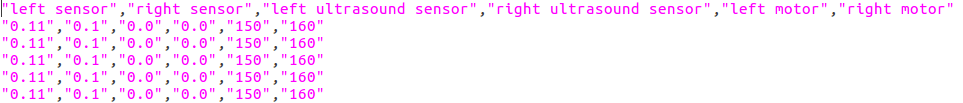
\includegraphics[width=\linewidth, height=25mm]{output_example.png}
	\caption{Output example} 
	\label{output_example}
\end{figure}
\\
First of all, we need to see in sensorimotor space how the motor and light values relate to each other. We know that as the robot goes to a light source, the light sensor value would go up to maximum of 1 for each sensors. We also know that the motor movement would go faster as the robot detects more light and vice versa. So we can safely assume that there are linear relationship between both of them. However, since we add an arena to our environment like in Figure \ref{arena}, we add some external variable to our experiment namely obstacles. 
\\\newline
We put together different initial angle for the robot and even only changing the starting position results in various graphs but there are still patterns that are noticeable. As we can see in Figure \ref{linear}, the general trajectories is going up linearly but sometimes you can see where the motor values go down which means it detects an obstacle in front of it and is backing up to avoid it. At the same time, we can also see that after the robot backs up, it detects more light that it has not before. Notice the green line where it does not go down at any moment means that the robot goes smoothly to the light without any hindrance whatsoever.
\begin{figure}[ht!]
	\centering
	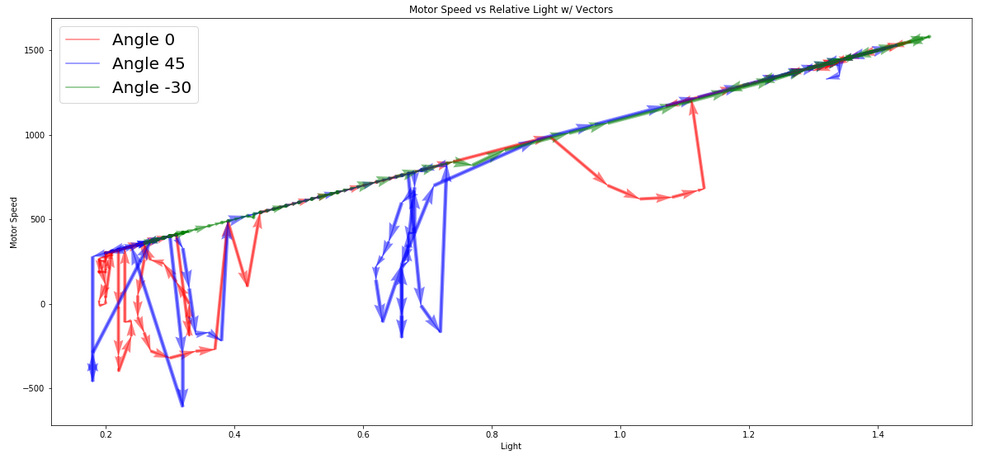
\includegraphics[width=100mm]{linear.png}
	\caption{linear} 
	\label{linear}
\end{figure}
\\\newline
Then, we want to see the state transition between the sensorimotor space. To do that, we need to normalize all values to between 0 and 1 then calculate the total with formula $dim1 + B * dim2 + B^2 * dim3 + \ldots$ where $dim1, \, dim2,$ and $ dim3$ is the sensor values that we want as the dimension and $B$ is the number of bins which in our case is 10. The total would result in integer values where \emph{total} $<$ $B^{number\, of\, dimensions}$. Finally, we digitize the total to bin with size $B$. This will result in an integer values between 0-($B-1$) for each dimensions. Note that we do not want transitions where a state goes to itself so we remove all these occurrences.
\\\newline
After visualising the graph above with $dim1$ = total sensor as x-axis and $dim2$ = total motor as y-axis, we determine that there are too much changes that we cannot see which one is important. Then, we figured that only visualising the most visited transition by a state will be much more interesting to look at. We did just that and it resulted in a less crowded transition graph and a more simple diagram. Also, we can see that some cycles appeared between state transitions. 
\begin{figure}[ht!]
	\centering
	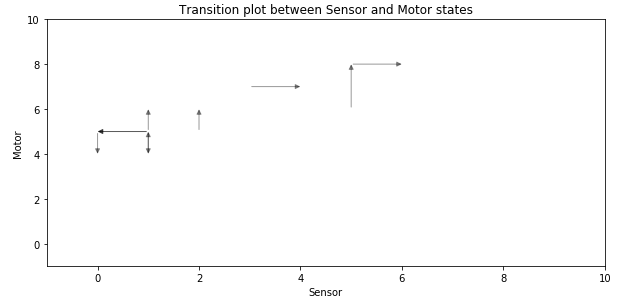
\includegraphics[width=100mm,height=45mm]{transition.png}
	\caption{State transition between total sensor and total motor}
	\label{transition}
\end{figure}
\\
\textbf{Note:} The higher the number, the bigger the original value is
\\\newline
With that in mind, we continue by asking why is there a cycle and see if that cycle will mean anything to our question of sensorimotor space. In other words, we are asking if that cycle is a habit that the robot develops when it is moving around in the arena or is it just random occurrences. To determine this, we first need to convert our state transitions list to a directed graph. It consists of the state itself as nodes and transitions as edges. We can use a function called \emph{simple\_cycles} in the \emph{networkx} library to check if cycle exists in our digraph. We also know that if a loop is detected in the state transition, each dimension of the loop is also a cycle by itself. Here is an example of the cycle with only 3 dimensions visualised. It will still form a cycle even in higher dimensions.
\begin{figure}[ht!]
	\centering
	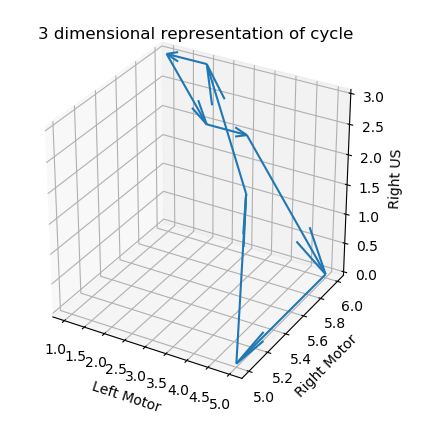
\includegraphics[width=60mm,height=40mm]{3d.png}
	\caption{3D cycle with reduced dimensions} 
	\label{3d}
\end{figure}
\\
We do not want a sequence where it just goes back and forth between its states, we called it line cycle, since it is not technically a "true cycle" (e.g. A B C B A). We want a cycle where it goes back to the original state without going to-and-fro (e.g. A B C A). To exclude such cycles, we use a technique called Principal Component Analysis (PCA). PCA is a statistical technique that is used to analyse possibly correlated values and explain these variables in a smaller dimension called principal components with as little loss of information as possible compared to original data \cite{pca}. We want to have at least two principal components for it to be a cycle that we can consider. 
\\\newline
Here is the matrix that we use for analyzing the data with PCA. It is an example of cycle in the form of 2D array with each column from left to right being left sensor, right sensor, left ultrasound, right ultrasound, left motor and right motor respectively and each row being the data point in the cycle.
\begin{figure}[ht!]
	\centering
	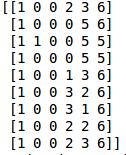
\includegraphics[width=30mm,height=20mm]{dimensions.png}
	\caption{2D array representation of cycle} \label{dimensions}
\end{figure}
\\\newline
We can see that the cycle in Figure \ref{dimensions} is varying only in column four and five so we know that there are going to be only two principal components. We can get the first principal component line by training the original data to see in which direction the most variance is. If we already got the first principal component line, we can use that line as our x-axis and transform our original cycle to make the first principal component.  
\\\newline
Using PCA on any data would reduce the dimensionality, in our case from six dimensions to mostly three or four. This is one way to exclude most of the line cycle since there is a high chance that a line cycle would just vary in one dimension which would result in one principal component only. This is not to say that this will rule out all of the line cycles since there is a case where it can vary in $>1$ dimensions but is still a line cycle. Figure \ref{pcacomparison} is a comparison between $>1$ and only one principal components
\begin{figure}[ht!]
	\centering
	\begin{subfigure}{.5\textwidth}
		\centering
		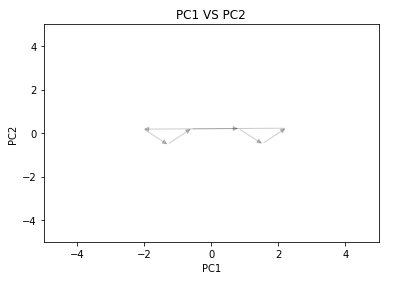
\includegraphics[width=.8\linewidth]{pcabiggerthan1.png}
		\caption{$>1$ principal component}
		\label{pcabiggerthan1}
	\end{subfigure}%
	\begin{subfigure}{.5\textwidth}
		\centering
		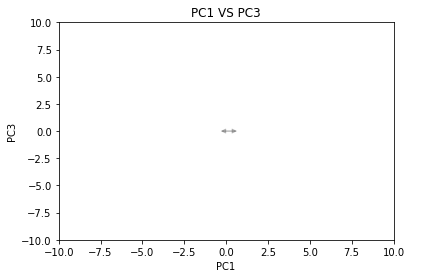
\includegraphics[width=.8\linewidth]{pca1.png}
		\caption{One principal component}
		\label{pca1}
	\end{subfigure}
	\caption{PCA Comparison}
	\label{pcacomparison}
\end{figure}
\section{Discussion}
First of all, note that all the experiment we have done is using a simple Braitenburg controller where the robot goal is to move toward a place where it detects more light and avoids obstacles in front of it. There are a more sophisticated controller or a manual one that we as the user can use with either keyboard or joystick but we will not discuss that since we have not experimented with that type of controller. There is no doubt that with using another type of controller will result in a much different and messier data than when using Braitenburg controller. Even though it is simple, it is enough for us to understand what is happening within the robot itself.
\\\newline
For the next step, we can start to discuss what does it mean by a habit-based robot. Habit, as defined by Merriam-Webster, is \emph{an acquired mode of behaviour that has become nearly or entirely involuntary} \cite{habit-definition}. In a sophisticated agent like a human, habit is acquired through learning from the previous experince of a same or similar situation. The more interesting question is if a simple agent like a robot can also learn any habit by itself. Much like a human, if the robot goes through a similar situation in the past, can it do the same activity subconsciously without the need to use its 'brain power'.\cite{matthew}
\\\newline
A cycle is an example of a habit that is formed by the agent moving through the sensorimotor trajectories but eventually goes back to its original position. If we somehow put this pattern that the robot did to train it, the possibility of using a learning algorithm where the robot can learn this pattern by itself without using its 'brain power' all over again every time is intriguing. However, this also means that the robot itself has to know about its spatial environment. If the robot does not recognise its surrounding, the robot will try to learn from the training set and see which one is the most suitable motor movement. The problem is, the concept of spatial environment could emerge only by exploring invariants in sensorimotor laws \cite{sensorimotor-theory}. The sensorimotor theory by itself would not allow a simple agent to understand the concept of space but only allowing it to know the notion of habit.

\section{Conclusion}
This whole project has been a treat, and I am glad to be able to do this project with the supervision from Matthew Egbert. He always support us with whatever we think is correct to do.
\\\newline
Regarding the project itself, there are broader concepts that we have not covered yet, and I think the result of this research will be useful when we understand and apply the idea of habit from robot to human.

\addcontentsline{toc}{section}{References}
\begin{thebibliography}{9}
	\bibitem{ev3dev}  
	Ev3dev Software / OS.
	\\\texttt{http://www.ev3dev.org} 
	
	\bibitem{ev3devWithPython}  
	Ev3dev with Python.
	\\\texttt{https://github.com/ev3dev/ev3dev-lang-python}
	
	\bibitem{habit-definition}
	Definition of habit.
	\\\texttt{https://www.merriam-webster.com/dictionary/habit}
	
	\bibitem{matthew}
	Matthew Egbert.
	\textit{Autonomous Patterns of Sensorimotor Activity.}
	\\\texttt{http://www.matthewegbert.com/projects/autonomous\_patterns\_of\_sensorimotor\_activity.html}
	
	\bibitem{sensorimotor-theory}
	J. Kevin O'Regan.
	\textit{Sensorimotor theory of consciousness.}
	\\\texttt{http://www.scholarpedia.org/article/Sensorimotor\_theory\_of\_consciousness}
	
	\bibitem{pca}
	Charles Zaiontz.
	\textit{Principal Component Analysis.}
	\\\texttt{http://www.real-statistics.com/multivariate-statistics/factor-analysis/principal-component-analysis/}
	
\end{thebibliography}
\end{document}